\documentclass[tikz, border=5mm]{standalone}
\usetikzlibrary{calc, arrows.meta, shapes.geometric}

\begin{document}
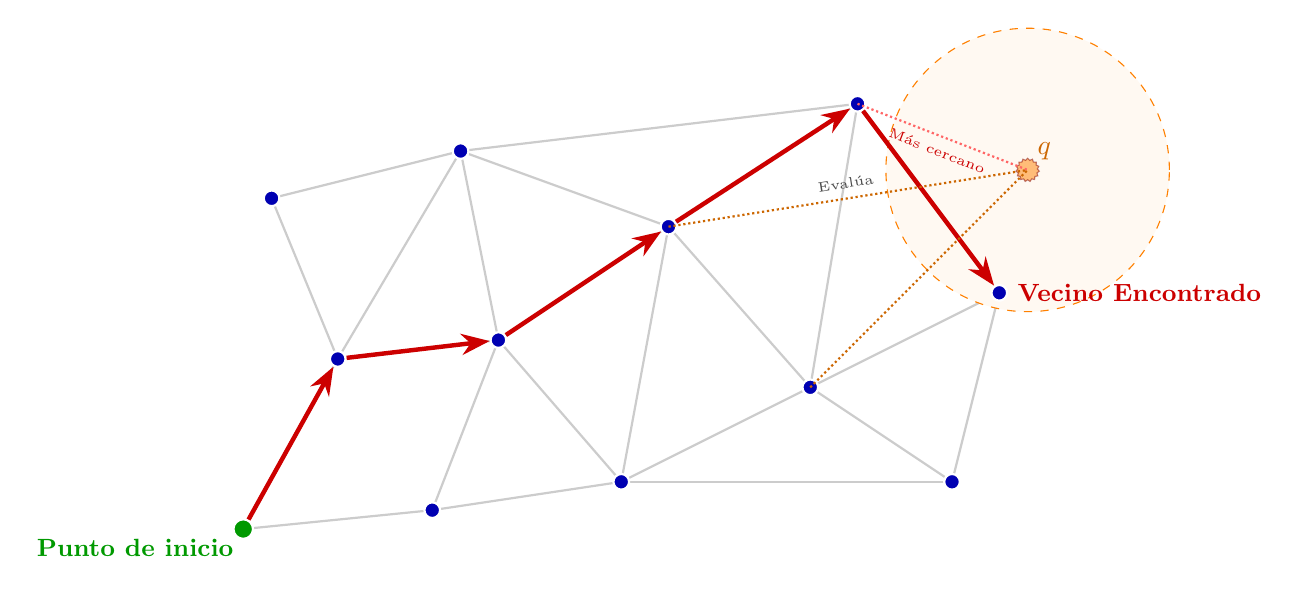
\begin{tikzpicture}[
    scale=1.2,
    % Definición de estilos
    node base/.style={circle, fill=blue!70!black, inner sep=2pt, draw=white, thick},
    edge knn/.style={thick, black!20}, % Aristas de fondo (vecindad)
    edge path/.style={->, >=Stealth, ultra thick, red!80!black}, % Ruta de búsqueda
    node entry/.style={circle, fill=green!60!black, inner sep=2.5pt, draw=white, thick},
    node query/.style={star, star points=15, star point ratio=1.2, fill=orange, opacity=0.5, inner sep=2.5pt, draw=red!50!black},
    eval line/.style={densely dotted, thick, orange!80!black} % Líneas de evaluación de distancia
]

    % =========================================================================
    % 1. Definición de Nodos del Grafo (Coordenadas Espaciales)
    % =========================================================================
    % Zona izquierda
    \coordinate (n1) at (0.5, 1.0); % Punto de entrada
    \coordinate (n2) at (1.5, 2.8);
    \coordinate (n3) at (0.8, 4.5);
    \coordinate (n4) at (2.5, 1.2);
    
    % Zona central
    \coordinate (n5) at (3.2, 3.0);
    \coordinate (n6) at (2.8, 5.0);
    \coordinate (n7) at (4.5, 1.5);
    \coordinate (n8) at (5.0, 4.2);
    
    % Zona derecha
    \coordinate (n9) at (6.5, 2.5);
    \coordinate (n10) at (7.0, 5.5);
    \coordinate (n11) at (8.5, 3.5); % Vecino más cercano real
    \coordinate (n12) at (8.0, 1.5);

    % =========================================================================
    % 2. Construcción de Aristas (Topología k-NN Aproximada)
    % =========================================================================
    % Conexiones locales para formar una malla navegable
    \draw[edge knn] (n1) -- (n2); \draw[edge knn] (n1) -- (n4);
    \draw[edge knn] (n2) -- (n3); \draw[edge knn] (n2) -- (n5); \draw[edge knn] (n2) -- (n6);
    \draw[edge knn] (n3) -- (n6);
    \draw[edge knn] (n4) -- (n5); \draw[edge knn] (n4) -- (n7);
    \draw[edge knn] (n5) -- (n6); \draw[edge knn] (n5) -- (n7); \draw[edge knn] (n5) -- (n8);
    \draw[edge knn] (n6) -- (n8); \draw[edge knn] (n6) -- (n10);
    \draw[edge knn] (n7) -- (n8); \draw[edge knn] (n7) -- (n9); \draw[edge knn] (n7) -- (n12);
    \draw[edge knn] (n8) -- (n9); \draw[edge knn] (n8) -- (n10);
    \draw[edge knn] (n9) -- (n10); \draw[edge knn] (n9) -- (n11); \draw[edge knn] (n9) -- (n12);
    \draw[edge knn] (n10) -- (n11);
    \draw[edge knn] (n11) -- (n12);

    % =========================================================================
    % 3. Punto de Consulta (Query) y Punto de Entrada
    % =========================================================================
    \coordinate (q) at (8.8, 4.8);
    
    % Área de vecindad de la consulta (Opcional, para ilustrar k=1)
    \draw[orange, dashed, fill=orange!5] (q) circle (1.5cm);

    % Dibujar nodos base (excepto el de entrada que se dibuja después)
    \foreach \i in {2,...,12} {
        \node[node base] (node\i) at (n\i) {};
    }
    
    % Nodo de Entrada (Entry Point)
    \node[node entry] (node1) at (n1) {};
    \node[below left, font=\bfseries\small, green!60!black] at (node1) {Punto de inicio};

    % Nodo de Consulta (q)
    \node[node query] (query) at (q) {};
    \node[above right, font=\bfseries, orange!80!black] at (query) {$q$};

    % =========================================================================
    % 4. Ilustración del Algoritmo de Ruteo Codicioso (Greedy Routing)
    % =========================================================================
    
    % Paso 1: n1 -> n2
    \draw[edge path] (node1) -- (node2);
    
    % Paso 2: Evaluación en n2 y salto a n5
    % (n2 evalúa a sus vecinos n3, n5, n6. n5 es el más cercano a q)
    \draw[edge path] (node2) -- (node5);
    
    % Paso 3: Evaluación en n5 y salto a n8
    \draw[edge path] (node5) -- (node8);
    
    % Paso 4: Evaluación en n8 y salto a n10
    \draw[edge path] (node8) -- (node10);
    
    % Paso 5: Evaluación en n10 y salto a n11 (Mínimo Local / Nearest Neighbor)
    \draw[edge path] (node10) -- (node11);

    % =========================================================================
    % 5. Detalles visuales de la evaluación en un salto específico (Ej. n8 -> n10)
    % =========================================================================
    % Mostrar cómo el algoritmo mide la distancia desde los vecinos de n8 hacia q
    \draw[eval line] (n8) -- (q) node[midway, sloped, above, font=\tiny, black!70] {Evalúa};
    \draw[eval line, red!60] (n10) -- (q) node[midway, sloped, below, font=\tiny, red!80!black] {Más cercano};
    \draw[eval line] (n9) -- (q);

    % Etiqueta del vecino final
    \node[right=3pt, font=\bfseries\small, red!80!black] at (node11) {Vecino Encontrado};

\end{tikzpicture}
\end{document}
